\section{Discussions on possible sources of the unknown excess} \label{sec-source}
On the basis of the obtained results, the possible explanation of the unknown excess below the $K^-pp$ threshold is discussed. The candidates are as follows:
\begin{enumerate}
\item Non-mesonic two-nucleon absorption processes
\item Mesonic two-nucleon and three-nucleon absorption processes
\item Formation of $K^-pp$ state
\end{enumerate}
Although these processes are still not well known both theoretically and experimentally, we compare the observed spectrum with expected spectra of the candidate processes. The expected spectra are evaluated with the simulation and the same analysis procedure as used for the data analysis. In the discussion, we use the $\Sigma$-decay subtracted spectrum shown in Fig. \ref{fig-ncswosigma}, since the $\Sigma$-decay events can be identified event by event as described in Sec. \ref{sec-sigmacut}.

\subsection{Non-mesonic two-nucleon absorption} \label{sec-2na}
Non-mesonic two-nucleon absorption reactions (NM2NA),
\begin{eqnarray}
K^-+``NN'' \to \Sigma/\Lambda +N.  \label{eq-nm2nr}
\end{eqnarray}
can produce high-energetic nucleons due to the large Q-values. 
In stopped-kaon experiments, the total non-mesonic multi-nucleon absorption rate was obtained to be 0.16 $\pm$ 0.03 on $^4$He\cite{Katz:1970ng}, but only $\sim$0.01 on deuteron\cite{VeldeWilquet:1977fh} using bubble chambers. Experiments using emulsion detectors also reported the rate to be as large as 0.2 on larger target\cite{Seki:1975hv}. Although several theoretical studies have been progressed\cite{Sekihara:2012bh,Onaga:1989vl}, the mechanism of multi-nucleon absorption processes is still not well understood. 
In the case of in-flight experiment, the reaction cross section of multi-nucleonic processes should be considerably small since the de Broglie wave length at 1 GeV/$c$ ($\sim$0.2 fm) is much shorter compared to the distance of two nucleons ($\sim$1.5 fm). However, their possible contributions are worth to be examined.
\\

Here, we consider not only ground state of $\Lambda, \Sigma$ but also hyperon resonances such as $\Sigma(1385), \Lambda(1405)$ and $\Lambda(1520)$ in NM2NA, namely, 
\begin{eqnarray}
K^- + {\rm ^3He} \to Y^{(*)} + N + N_s, 
\end{eqnarray}
where $Y^{(*)}$ and $N_s$ denote hyperon or hyperon resonance and a spectator nucleon in helium-3, respectively. All the possible charge combinations are listed in Table \ref{tab-nm2n}. 
Once the reaction angle is determined, the emitted nucleon has monochromatic momentum except for the smearing by the Fermi motion. Thus they make peak structures in the neutron spectrum as shown in Fig. \ref{fig-mmnm2n}, where the simulated spectra of NM2NA are compared with the experimental spectrum. The relative reaction cross section of each charge combination is assumed to be equal for the simplicity. It should be noted that we use the Breit-Wigner distributions with PDG masses and widths to describe intrinsic resonance shapes of the hyperons. 

Possible contributions of NM2NA are discussed in the following.
\begin{table}[]
\caption[List of non-mesonic two nucleon absorption processes]{List of non-mesonic two nucleon absorption processes. The estimations are given as by the sum of differential cross sections at $\theta^N_{lab}=0^\circ$ for all charge combinations.}
\begin{center}
\begin{tabular}{llcc} 
\hline\hline
mode	&	charge combinations	&	\# of comb.	&	estimation	\\
\hline							
$\Lambda N$	&	$\Lambda n p_s$, $\Lambda p n_s$	&	2	&	$<$0.1 mb/sr	\\
$\Sigma N$	&	$\Sigma^- p p_s$, $\Sigma^0 n p_s$, $\Sigma^0 p n_s$, $\Sigma^+ n n_s$	&	4	&	$<$0.1 mb/sr	\\
\raisebox{1.5ex}{$\Sigma(1385) N$}	&	\shortstack{$\Sigma(1385)^- p p_s$, $\Sigma(1385)^0 n p_s$, \\ $\Sigma(1385)^0 p n_s$, $\Sigma(1385)^+ n n_s$}	&	4	&	$<$0.1 mb/sr	\\
$\Lambda(1405) N$	&	$\Lambda(1405) n p_s$, $\Lambda(1405) p n_s$	&	2	&	11 mb/sr	\\
$\Lambda(1520) N$	&	$\Lambda(1520) n p_s$, $\Lambda(1520) p n_s$	&	2	&	4 mb/sr	\\
\hline \hline
\end{tabular}
\end{center}
\label{tab-nm2n}
\end{table}%

\begin{figure}[]
\begin{center}
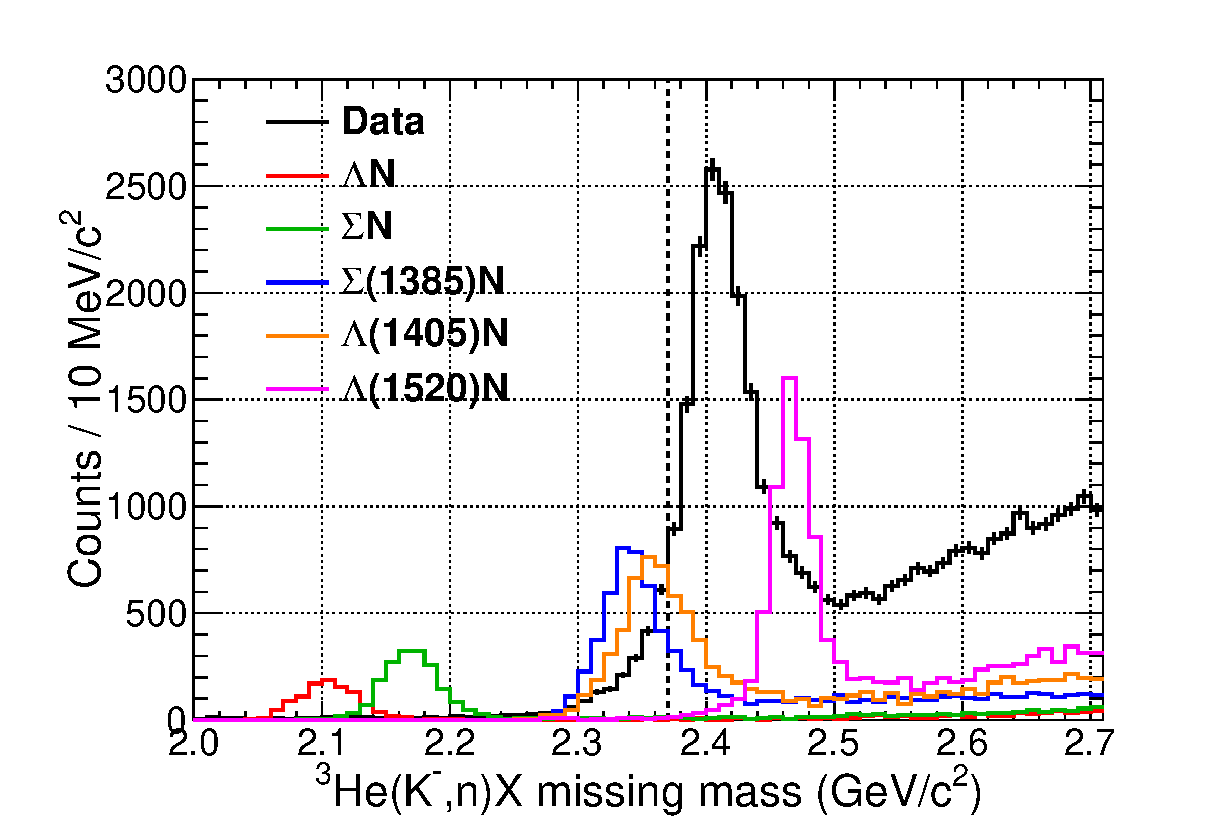
\includegraphics[width=12cm]{./fig/mm-nm2n.eps}
\caption[Simulated neutron spectra in NM2NA.]{Simulated neutron spectra in NM2NA. For each branch, the number of generated events corresponds to 20 mb/sr at $\theta_{lab}=0^\circ$.}
\label{fig-mmnm2n}
\end{center}
\end{figure}  

\subsubsection{$\Lambda N$ and $\Sigma N$ branches}
In the $\Lambda N$ and the $\Sigma N$ branches in NM2NA, both primary neutrons and neutrons from hyperon decays contribute to the deep bound region around 2.1$\sim$2.2 GeV/$c^2$ as shown in Fig. \ref{fig-mmnm2n}. The experimental spectrum have reveals no significant structure in such region, which indicates the contributions of the $\Lambda N$ and the $\Sigma N$ branches of NM2NA are quite limited. This fact is consistent to the result of KEK PS-E548\cite{Kishimoto:2007kr}(Fig. \ref{fig-e548kishimoto}). They found no significant contribution from reaction (\ref{eq-nm2nr}) in $^{12}$C$(K^-,N)$ reactions at 1 GeV/$c$. Rough estimations of the upper limit for the reaction cross sections were done by fitting histogram with their simulated line shape and continuous background. %They were estimated to be xx mb/sr, xx mb/sr at $\theta_{lab}$=0$^\circ$ for $\Lambda N$ and $\Sigma N$, respectively. 

\subsubsection{$\Sigma^* N$ and $\Lambda^* N$ branches}
In NM2NA which produce hyperon resonances, contributions of the primary neutrons appear at the tail of the observed quasi-free peak, while neutrons from their decays make broad continuum in higher missing-mass region.

Now we simply assume the tail structure is fully composed of the $Y^* N$ branches in NM2NA. The main shape of the quasi-free peak is assumed to be the same as the $K^0_s$ tagged spectrum. Then the neutron spectrum was fitted by the four components with four free parameters which define their intensities. The fitting result is shown in Fig. \ref{fig-ystar2n}. We obtained rather large cross section of $\sim$5 mb/sr and $\sim$2 mb/sr at $\theta_{lab}=0^\circ$ for the $\Lambda(1405)n$, and the $\Lambda(1520)n$ branches, respectively, while the contribution of the $\Sigma(1385)n$ branch was much suppressed. Thus, the obtained yields for $\Lambda^* N$ branches give upper limit of their contribution. 
\\

%\subsubsection{Discussions on the $\Sigma^* N$ and $\Lambda^* N$ branches}
%In our data, it is almost impossible to restrict the contribution of these processes any further. Especially, the $\Lambda(1405)n$ branch of NM2NA and the $K^-pp$ formation decaying into $\pi\Sigma$ final state are kinematically similar reactions. We need much more statistics to distinguish them in an exclusive analysis. 
Here, we discuss whether the large contribution of the $\Lambda(1405)n$ branch in NM2NA is reasonable or not, by referring other experimental and theoretical information.
A previous in-flight kaon experiment by Braun {\it et. al.} using a deuterium bubble chamber at 834 MeV/$c$ reported sub mb total cross sections of $\Sigma(1385)^-p$($\sim$0.3 mb), $\Lambda(1405)n$ ($\sim$0.4 mb), and $\Lambda(1520)n$ ($\sim$0.9 mb) final states\cite{Braun:1977fy}. In the theoretical side, there is a calculation of the $d(K^-,n)\Lambda(1405)/\Sigma(1385)$ reactions, which predicts the enhancement of $\Lambda(1405)$ production at forward angle\cite{YamagataSekihara:2013jh}. However, they evaluated the differential cross section of $\Lambda(1405)n$ final state to be only $\sim$0.5 mb/sr at $\theta_{lab}=0^\circ$, while that of $\Sigma(1385)$ to be one order of magnitude smaller. Therefore, the dominance of $\Lambda(1405)n$ branch against $\Sigma(1385)n$ branch is reasonable, while more than 1 mb/sr cross section of $\Lambda(1405)n$ branch seems unreasonable.

Another point is the large cross section compared to $\Lambda(1520)$ branch. The production cross section of $\Lambda(1520)$ was measured to be approximately 5 times larger than that of $\Lambda(1405)$  in the elementally processes (see Table \ref{tab-kpreaction}) and approximately 2 times larger in NM2NA on a deuteron target, while we obtained less than half yileds of $\Lambda(1520)n$ at maximum compared to $\Lambda(1405)n$. 
%Therefore, these are also different from our data with helium-3 target.
\\

In summary, the assumption that the tail structure below the threshold can be fully reproduced with $Y^*n$ branches of NM2NA seems not reasonable in view of the obtained large cross section of $\Lambda(1405)n$ branch, but cannot be excluded by the present data only. Note that the peak position and the resonance shape of $\Lambda(1405)$ would have a large influence on the quantitative discussion.
\\

Anyway, with the semi-inclusive analysis, the information on each branch in NM2NA could not be extracted more precisely. In particular the $\Lambda(1405)n$ branch and $K^-pp$ formation cannot be distinguished with the $^3$He$(K^-,n)X$ missing-mass spectrum. We need much more statistics to achieve the exclusive analysis by reconstructing $\pi\Sigma$, $\pi\Sigma p$, and $\Lambda p$ final states.
\begin{figure}
\begin{center}
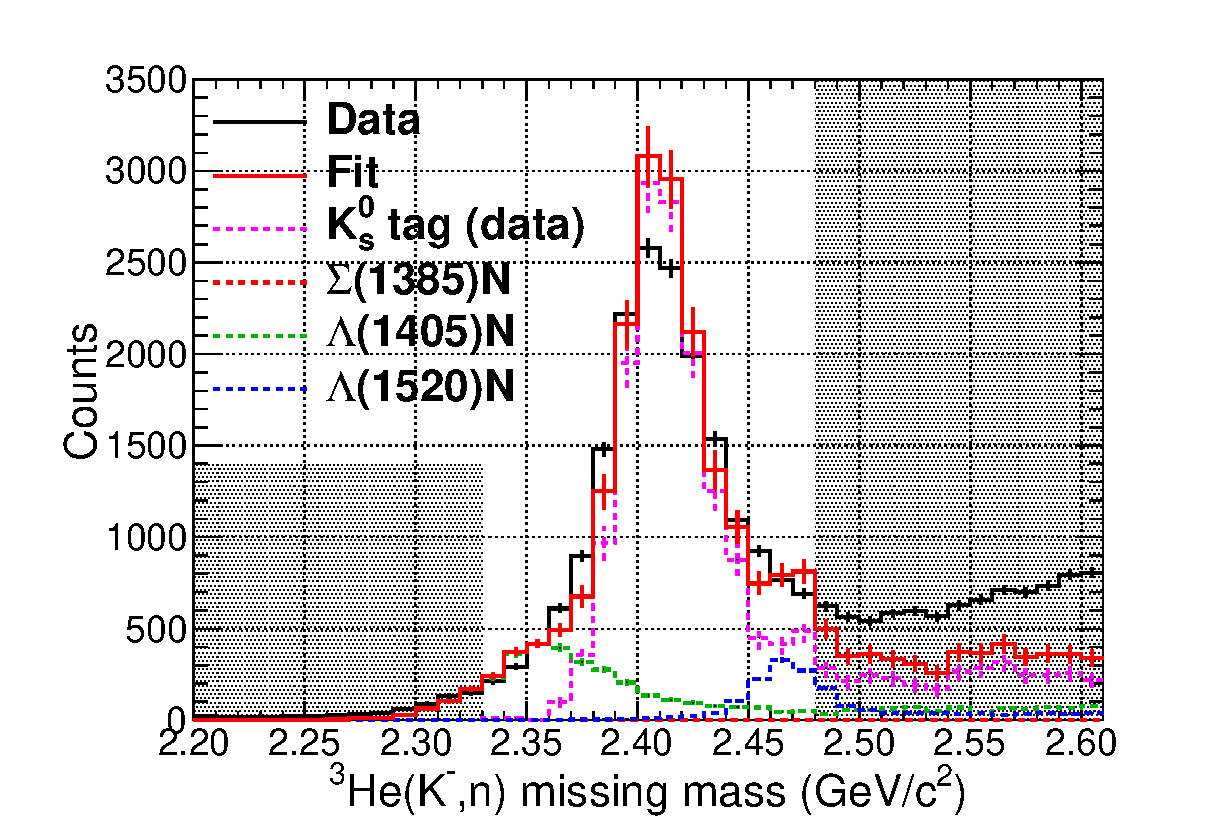
\includegraphics[width=12cm]{./fig/mm-ystar2nfit.eps}
\caption[Neutron missing-mass spectrum fitted with the simulated spectra of the $Y^*N$ branches and the $K_s^0$-tagged spectrum.]{Neutron missing-mass spectrum fitted with the simulated spectra of the $Y^*N$ branches and the $K_s^0$-tagged spectrum. The hatched regions were excluded from the fitting.}
\label{fig-ystar2n}
\end{center}
\end{figure}  


\subsection{Mesonic two-nucleon absorption and three-nucleon absorption\label{sec-multin}}
There would be also two-nucleon absorption reactions (2NA) associated with pion(s) and three-nucleon absorption reactions (3NA) such as,
\begin{eqnarray}
K^- + {\rm ^3He} \to Y + N + \pi + N_s \label{eq-2nr} \\
K^- + {\rm ^3He} \to Y + N + N + (\pi)  \label{eq-3nr}.
\end{eqnarray}
Here we consider the processes with up to three pions for 2NA and with up to two pions for 3NA as listed in Table \ref{tab-pi2n} and Table \ref{tab-3n}, respectively. If the final state particles distribute uniformly in the phase space, these processes would make broad continuums in the neutron missing mass spectrum as shown in Fig. \ref{fig-mmpi2n}(left) and \ref{fig-mm3n}(left). In the simulation, the relative reaction cross section of each combination is assumed to be equal for the simplicity. 

In these reactions, $\Lambda p$ pairs are expected to be reconstructed with the CDS. Note that $\Sigma^0$ also produces $\Lambda$ via its decay into $\Lambda\gamma$. The simulated spectra of $\Lambda p$ invariant masses are also compared with the data as shown in Fig. \ref{fig-mmpi2n}(right) and Fig. \ref{fig-mm3n}(right). The event selection and the normalization of the $\Lambda p$ events are described in Appendix C.

\begin{table}[]
\caption[List of the mesonic two-nucleon absorption processes. ]{List of the mesonic two-nucleon absorption processes. The yields are estimated by fitting $\Lambda p$ spectra, and  are given as the sum of total cross sections of all charge combinations.}
\begin{center}
\begin{tabular}{llccl} 
\hline\hline
branch	&	charge combinations	&	\# of comb.	&	estimation	\\
\hline							
$\Lambda N\pi$	&	$\Lambda n \pi^0 p_s$, $\Lambda p \pi^- p_s$,  $\Lambda p \pi^0 n_s$, $\Lambda n \pi^+ n_s$ 	&	4	&	$<$0.1 mb	\\
\hline							
$\Lambda N\pi\pi$	&	\shortstack{$\Lambda n (\pi\pi)^0 p_s$, $\Lambda p (\pi\pi)^-p_s$, \\ $\Lambda p (\pi\pi)^0 n_s$, $\Lambda n (\pi\pi)^+ n_s$}	&	6	&	$<$0.1 mb	\\
\hline							
$\Lambda N\pi\pi\pi$	&	\shortstack{$\Lambda n (\pi\pi\pi)^0 p_s$, $\Lambda p (\pi\pi\pi)^-p_s$, \\ $\Lambda p (\pi\pi\pi)^0 n_s$, $\Lambda n (\pi\pi\pi)^+ n_s$}	&	8	&	34 mb	\\
\hline							
$\Sigma N\pi$	&	\shortstack{$\Sigma^- p \pi^0 p_s$, $\Sigma^- n \pi^+ p_s$, $\Sigma^0 n \pi^0 p_s$,\\ $\Sigma^0 p \pi^- p_s$, $\Sigma^+ n \pi^- p_s$,\\ $\Sigma^- p \pi^+ n_s$, $\Sigma^0 p \pi^0 n_s$, $\Sigma^0 n \pi^+ n_s$, \\ $\Sigma^+ n \pi^0 n_s$, $\Sigma^+ p \pi^- n_s$}	&	10	&	$<$0.1 mb	\\
\hline							
$\Sigma N\pi\pi$	&	\shortstack{$\Sigma^- p (\pi\pi)^0 p_s$, $\Sigma^- n (\pi\pi)^+ p_s$, $\Sigma^0 n (\pi\pi)^0 p_s$,\\ $\Sigma^0 p (\pi\pi)^- p_s$, $\Sigma^+ n (\pi\pi)^- p_s$, $\Sigma^+ p \pi^-\pi^- p_s$,\\ $\Sigma^- p (\pi\pi)^+ n_s$, $\Sigma^0 p (\pi\pi)^0 n_s$, $\Sigma^0 n (\pi\pi)^+ n_s$, \\ $\Sigma^+ n (\pi\pi)^0 n_s$, $\Sigma^+ p (\pi\pi)^- n_s$, $\Sigma^- n \pi^+\pi^+ n_s$}	&	16	&	$<$0.1 mb	\\
\hline							
$\Sigma N\pi\pi\pi$	&	\shortstack{$\Sigma^- p (\pi\pi\pi)^0 p_s$, $\Sigma^- n (\pi\pi\pi)^+ p_s$, $\Sigma^0 n (\pi\pi\pi)^0 p_s$,\\ $\Sigma^0 p (\pi\pi\pi)^- p_s$, $\Sigma^+ n (\pi\pi\pi)^- p_s$, $\Sigma^+ p \pi^-\pi^-\pi^0 p_s$,\\ $\Sigma^- p (\pi\pi\pi)^+ n_s$, $\Sigma^0 p (\pi\pi\pi)^0 n_s$, $\Sigma^0 n (\pi\pi\pi)^+ n_s$, \\ $\Sigma^+ n (\pi\pi\pi)^0 n_s$, $\Sigma^+ p (\pi\pi\pi)^- n_s$, $\Sigma^- n \pi^+\pi^+\pi^0 n_s$}	&	22	&	86 mb	\\\hline \hline
\end{tabular}
\end{center}
\label{tab-pi2n}
\end{table}%

\begin{table}[]
\caption[List of the three-nucleon absorption processes. ]{List of the three-nucleon absorption processes. The yields are estimated by fitting $\Lambda p$ spectra, and  are given as the sum of total cross sections of all charge combinations.}
\begin{center}
\begin{tabular}{llcc} 
\hline\hline
branch	&	charge combinations	&	\# of comb.	&	estimation	\\
\hline							
$\Lambda NN$	&	$\Lambda n p$	&	1	&	0.2 mb	\\
$\Lambda NN\pi$	&	$\Lambda n p \pi^0$, $\Lambda p p \pi^- $,  $\Lambda n n \pi^+ $ 	&	3	&	2 mb	\\
\hline							
$\Lambda NN\pi\pi$	&	$\Lambda n p (\pi\pi)^0$, $\Lambda p p (\pi\pi)^- $,  $\Lambda n n (\pi\pi)^+ $ 	&	4	&	$<$ 0.1 mb	\\
\hline							
$\Sigma NN$	&	$\Sigma^- p p$, $\Sigma^0 n p$, $\Sigma^+ n n$	&	3	&	0.2 mb	\\
\hline							
$\Sigma NN\pi$	&	\shortstack{$\Sigma^- p p \pi^0$, $\Sigma^- n p \pi^+$,\\ $\Sigma^0 p p \pi^-$, $\Sigma^0 p n \pi^0$, $\Sigma^0 n n \pi^+$,\\$\Sigma^+ n p \pi^-$, $\Sigma^+ n n \pi^0 $}	&	7	&	3 mb	\\
\hline							
$\Sigma NN\pi\pi$	&	\shortstack{$\Sigma^- p p (\pi\pi)^0$, $\Sigma^- n p (\pi\pi)^+$, $\Sigma^- n n \pi^+\pi^+$,\\ $\Sigma^0 p p (\pi\pi)^-$, $\Sigma^0 p n (\pi\pi)^0$, $\Sigma^0 n n (\pi\pi)^+$,\\$\Sigma^+ n p (\pi\pi)^-$, $\Sigma^+ n n (\pi\pi)^0 $, $\Sigma^+ p p \pi^-\pi^-$}	&	12	&	31 mb	\\
\hline \hline
\end{tabular}
\end{center}
\label{tab-3n}
\end{table}%

\begin{figure}[]
\begin{center}
\includegraphics[width=\columnwidth]{./fig/mm-pi2n.eps}
\caption[Simulated spectra of mesonic 2NA processes.]{Simulated spectra of mesonic 2NA (left) in the neutron missing-mass spectrum and (right) in the $\Lambda p$ missing-mass spectrum. The yield of each simulated spectrum is normalized to 10 mb total cross section. }
\label{fig-mmpi2n}
%\end{figure}  
%\begin{figure}[]
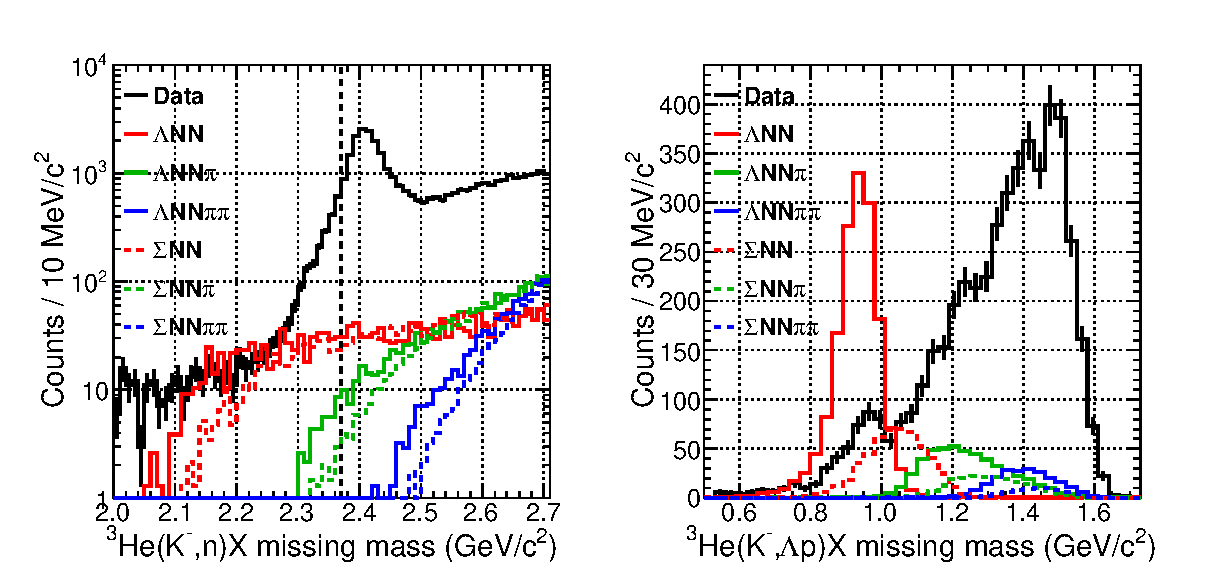
\includegraphics[width=\columnwidth]{./fig/mm-3n.eps}
\caption[Simulated spectra of 3NA processes.]{Simulated spectra of 3NA (left) in the neutron missing-mass spectrum and (right) in the $\Lambda p$ missing-mass spectrum. The yield of each simulated spectrum is normalized to (left) 10 mb and (right) 1 mb total cross section.}
\label{fig-mm3n}
\end{center}
\end{figure}  


\subsubsection{Estimation of the contribution in a simple assumption}
Since the $\Lambda p$ pairs can be produced in the two- or the three-nucleon processes only, we can restrict the yield of such processes from the distribution of the $\Lambda p$ events. Although the observed $\Lambda p$ events may contain signals of NM2NA and $S=-1$ bound/resonance states including $K^-pp$, we assume all observed events are generated by the uncorrelated mesonic 2NA and 3NA to evaluate the upper limits of the contributions from those processes. We fit the $^3$He$(K^-,\Lambda p)X$ missing-mass and the $\Lambda p$ invariant-mass spectra with simulated ones simultaneously as shown in Fig. \ref{fig-mmlpfit} . The yields of the 12 processes are determined by the fitting, where the fitting region are from 0.7 to 1.6 GeV/$c^2$ and from 2.05 to 2.7 GeV/$c^2$ for the missing-mass and invariant-mass, respectively. The systematic errors of the yields are estimated to be $\sim$ 20\% by changing the initial parameters of the fit and the fitting regions. By using obtained yields, their contributions to the $^3$He$(K^-,n)X$ missing-mass spectrum are evaluated as shown in Fig. \ref{fig-mm2n3nbg}.

Although the estimation method is too simple to determine the cross sections of each process, it is enough to evaluate the contribution in the $K^-pp$ bound region of the missing mass spectrum, since the $^3$He$(K^-,n)X$ missing-mass distributions of the multi-nucleon absorption processes would be highly correlated with the $\Lambda p$ distributions. The obtained yields of uncorrelated mesonic 2NA and 3NA is two orders of magnitude smaller than that of the excess, which clearly suggests such processes cannot explain the observed excess.

\begin{figure}[]
\begin{center}
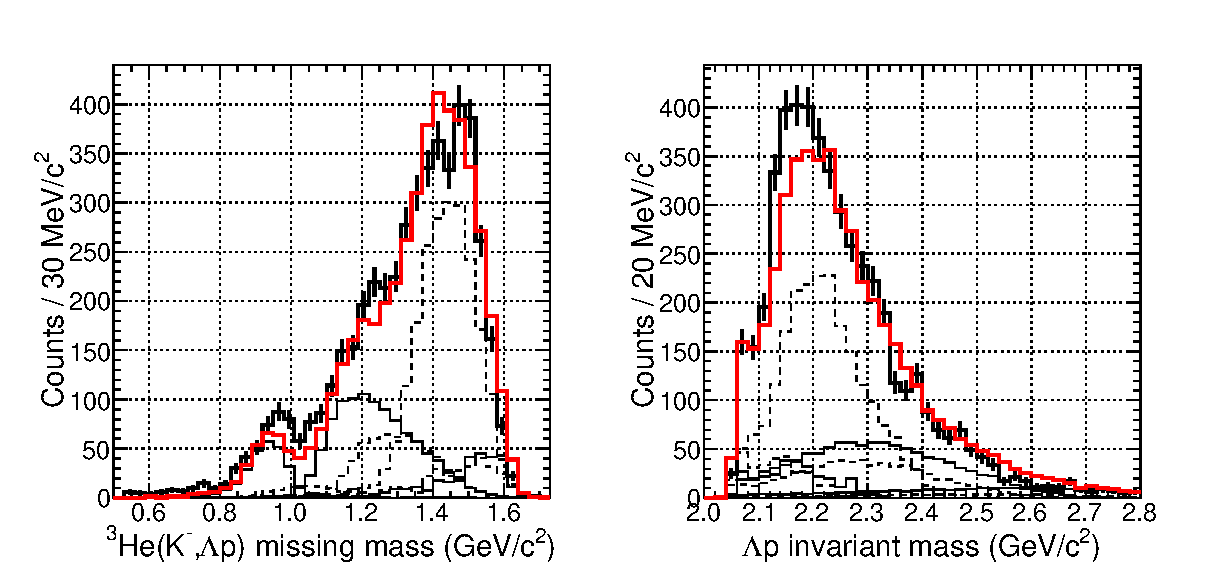
\includegraphics[width=\columnwidth]{./fig/mm-lpfit.eps}
\caption[$^3$He($K^-,\Lambda p)X$ missing-mass and $\Lambda p$ invariant-mass spectra.]{(left) $^3$He($K^-,\Lambda p)X$ missing-mass and (right) $\Lambda p$ invariant-mass spectra. They are fitted with the simulated spectra simultaneously. The thick black and the red histograms represent the data and the fitting result, respectively.}
\label{fig-mmlpfit}
%\end{figure}  
%\begin{figure}[]
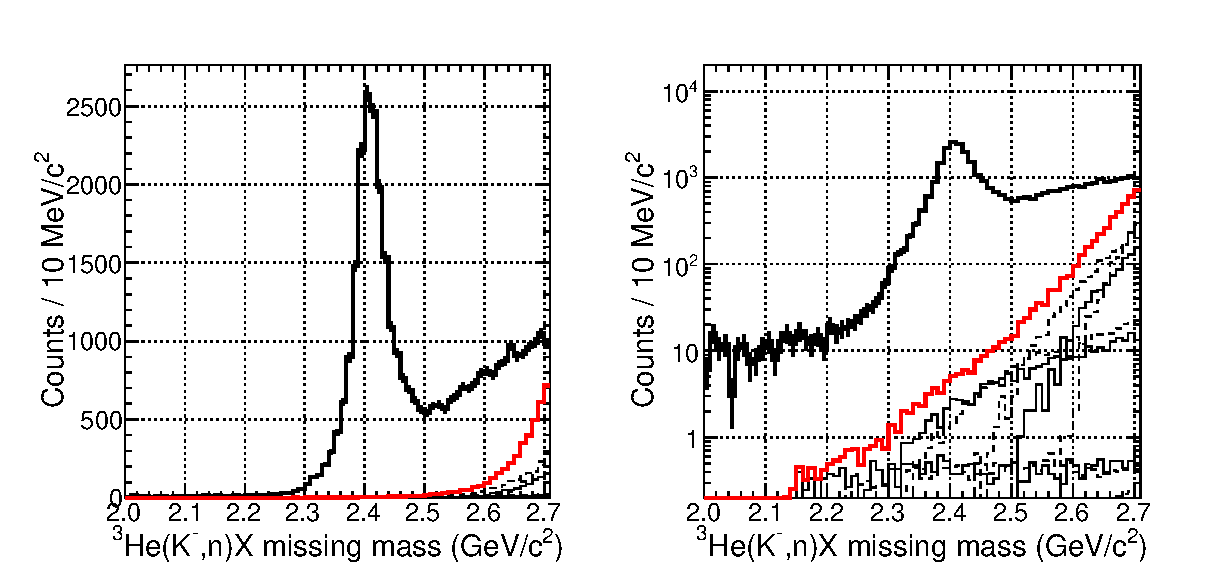
\includegraphics[width=\columnwidth]{./fig/mm-2n3nbg.eps}
\caption[$^3$He($K^-,n)X$ missing-mass spectra of mesonic 2NA and 3NA.]{$^3$He($K^-,n)X$ missing-mass spectra of mesonic 2NA and 3NA (left) in linear scale and (right) in log scale. The thick black and the red histograms represent the data and the obtained result, respectively.}
\label{fig-mm2n3nbg}
\end{center}
\end{figure} 
